% Chapter 1

\chapter{Data Set} % Main chapter title

\label{Chapter3} % For referencing the chapter elsewhere,  use \ref{Chapter1} 
\lhead{Chapter 3. \emph{Data Set}} % This is for the header on each page - perhaps a shortened title
%----------------------------------------------------------------------------------------
The social network meta data related to images can be made the basis image classification tasks and many times can outperform image content based methods \cite{Jure}. For the validation of this hypothesis, we needed a well labeled image data, which should also have a sufficient possibility of expanding it in social dimension. The data must have some ground truth provided by human annotators or by some standard benchmarks.\\
\hspace*{1cm} Most of the Large Scale Image Benchmarks are usually fabricated by the use of the vast sphere of images available on web. These images are  majorly the part of social media holders like Pin-interest, Flicker, Facebook. After exploring the available image benchmarks, we narrowed our focus on the following four well established benchmarks, because these were created of flicker images and by implementing the flicker APIs on available information, we could extract enough social meta data about the images:\\
\begin{itemize}
\item The PASCAL Visual Object Challenge ('PASCAL') \cite{pascal} 
\item The MIR Flickr Retrieval Evaluation ('MIR')\cite{MIR}
\item The ImageCLEF Annotation Task ('CLEF')\cite{CLEF}
\item The NUS Web Image Database ('NUS')\cite{NUS} 
\end{itemize}
The creators of these data-set had obtained labels through crowd-sourcing, the ficker users  or communities. The labels range from object based categories like \textit{person} or \textit{bicycle}, to subjective concepts like \textit{Aesthetic\_ Impression}. These labels satisfies the desired ground truth constraint for our classification process. We, therefore, use these labels as a classification base for our analysis.\\
\section{Description of Data sets}
The PASCAL Visual Object Challenge ('PASCAL') consists of over 12,000 images collected since 2007, with additional images added each year \cite{pascal}. Flickr sources were available only for training images, and for the test images from 2007. There were total of 11,197 images, for which flicker sources were available.\\
The MIR Flickr Retrieval Evaluation ('MIR') \cite{MIR} consists of one million images, 25,000 of which have been annotated. Flickr sources were available for 15,203 of the annotated images.\\
The ImageCLEF Annotation Task ('CLEF') \cite{CLEF} uses a subset of 18,000 images from the MIR data set, but it has more varied tagging annotation. There were total of 4,807 images, for which flicker sources were available. \\ 
The NUS Web Image Database ('NUS')  \cite{NUS} consists of approximately 270,000 Images. Flickr sources are available for all images.
\section{Augmentation of Social Meta-data}
Flicker Sources of above data sets were provided by the data set creators. We used the possible flicker APIs and tried to obtain the maximum meta data for each photo instance. The information, we could extract out were
\begin{itemize}
\item 	The photo itself
\item 	Photo data,
\begin{itemize}
\item Title
\item Description
\item Location
\item Time stamp
\item View count
\item Upload date
\end{itemize}
\item 	User information, including the uploader's name, username, location, their network of contacts, etc.
\item 	Photo tags, and the user who provided each tag
\item 	Groups to which the image was submitted 
\item 	Collections (or sets) in which the photo was included 
\item 	Galleries in which the photo was included 
\item 	 Comment threads for each image instance
\end{itemize}
We considered only the images which have all the above data available, which is roughly 90\% of the images for which the URL Source was available.
\section{Preliminary Observation of Data set}
We also did some observation while extracting data. We would like to give those observations at this stage because those will help us describe the inferences and results.\\
\begin{center}
\begin{figure}
\centering
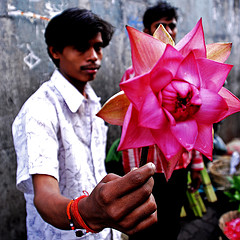
\includegraphics[width=3cm, height=3cm]{./Pictures/MIR/1.jpg}
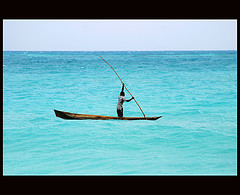
\includegraphics[width=3cm, height=3cm]{./Pictures/MIR/2.jpg}
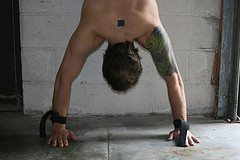
\includegraphics[width=3cm, height=3cm]{./Pictures/MIR/3.jpg} \\
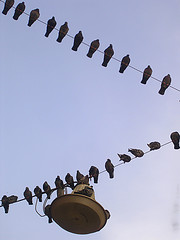
\includegraphics[width=3cm, height=3cm]{./Pictures/MIR/4.jpg}
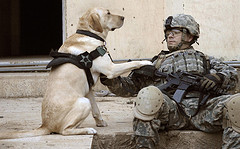
\includegraphics[width=3cm, height=3cm]{./Pictures/MIR/5.jpg}
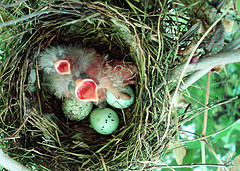
\includegraphics[width=3cm, height=3cm]{./Pictures/MIR/6.jpg}
\caption{Image MIR Examples}
\label{fig:Image MIR Examples}
\end{figure}
\end{center}
\vspace*{1cm}
\begin{center}
\begin{figure}
\centering
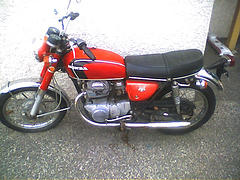
\includegraphics[width=3cm, height=3cm]{./Pictures/PASCAL/1.jpg}
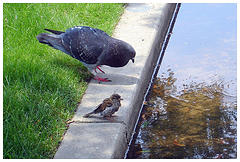
\includegraphics[width=3cm, height=3cm]{./Pictures/PASCAL/2.jpg}
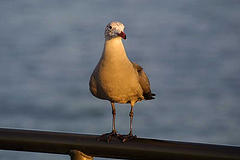
\includegraphics[width=3cm, height=3cm]{./Pictures/PASCAL/3.jpg} \\
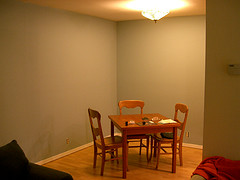
\includegraphics[width=3cm, height=3cm]{./Pictures/PASCAL/4.jpg}
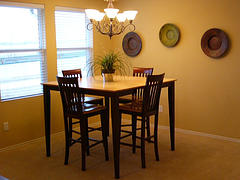
\includegraphics[width=3cm, height=3cm]{./Pictures/PASCAL/5.jpg}
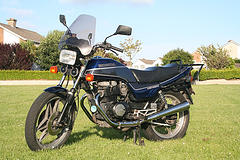
\includegraphics[width=3cm, height=3cm]{./Pictures/PASCAL/6.jpg}
\caption{Image PASCAL Examples}
\label{fig:Image PASCAL Examples}
\end{figure}
\end{center}
The statistics obtained from enriching the images and elementary statistical analysis of image properties reveals that there is a large difference between the data-sets, for example PASCAL has least tags and comments compare to all other data-sets, because it is made up of less interesting images. The NUS Data Set favors the highly popular images as we can see that it has the highest tag vs image ratio of 19.4. Th  images are highly tagged, have large number of comments and are submitted to many group. The MIR has 17$+$ tags comments showing that it contains 'interesting images' \cite{MIR} \\
%\[Attach some SCATTER PLOTS if you need\]\\
\begin{center}
\begin{figure}
\centering
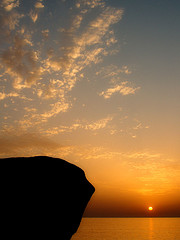
\includegraphics[width=3cm, height=3cm]{./Pictures/CLEF/1.jpg}
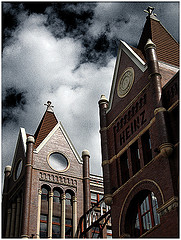
\includegraphics[width=3cm, height=3cm]{./Pictures/CLEF/2.jpg}
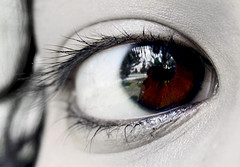
\includegraphics[width=3cm, height=3cm]{./Pictures/CLEF/3.jpg} \\
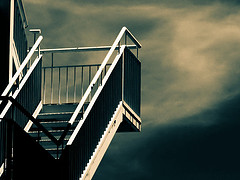
\includegraphics[width=3cm, height=3cm]{./Pictures/CLEF/4.jpg}
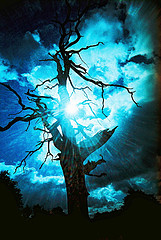
\includegraphics[width=3cm, height=3cm]{./Pictures/CLEF/5.jpg}
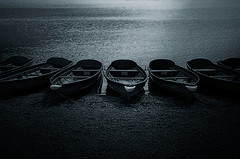
\includegraphics[width=3cm, height=3cm]{./Pictures/CLEF/6.jpg}
\caption{Image CLEF Examples}
\label{fig:Image CLEF Examples}
\end{figure}
\end{center}
\vspace*{1cm}
\begin{center}
\begin{figure}
\centering
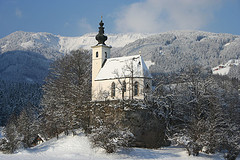
\includegraphics[width=3cm, height=3cm]{./Pictures/NUS/1.jpg}
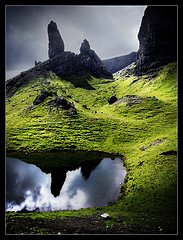
\includegraphics[width=3cm, height=3cm]{./Pictures/NUS/2.jpg}
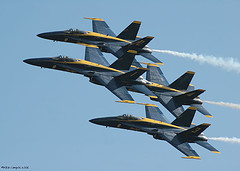
\includegraphics[width=3cm, height=3cm]{./Pictures/NUS/3.jpg} \\
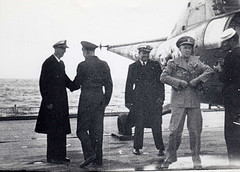
\includegraphics[width=3cm, height=3cm]{./Pictures/NUS/4.jpg}
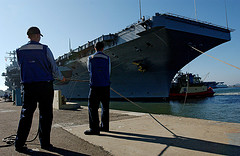
\includegraphics[width=3cm, height=3cm]{./Pictures/NUS/5.jpg}
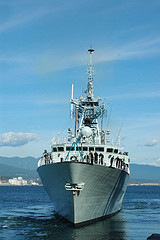
\includegraphics[width=3cm, height=3cm]{./Pictures/NUS/6.jpg}
\caption{Image NUS Examples}
\label{fig:Image NUS Examples}
\end{figure}
\end{center}
\vspace*{1cm}
\section{Label Selection for Classification Problem}
Due to constraint of presence of less number of images for some particular labels and balanced learning, we have to selectively choose the labels for our Classification Problem. \\
For eq. CLEF has 99 labels and some labels have image instances of less than 17 images, so doing a learning and testing on such small set is out of question. We, therefore, in case of CLEF select 20 Labels which have sufficient data. Similarly for NUS, because of some computational constraints and data availability, we reduce our computation for 12 labels. Following table shows the labels, which are considered in the whole classification problem. \\
%-------------------- Table example ------------------------------
\begin{table}[ht]
\caption{Labels} % title of Table
\centering % used for centering table
\begin{tabular}{|c|p{2cm}|p{7cm}| } % centered columns (4 columns)
\hline\hline %inserts double horizontal lines
DataSet & Number of Labels Selected & Labels \\ [0.5ex] % inserts table 
%heading
\hline % inserts single horizontal line
NUS & 10 & animal, coral, dancing, harbor, military, mountain, snow, statue, tattoo, temple, waterfall, wedding \\  [1ex]
PASCAL & 20 & aeroplane, bicycle, bird, boat, bottle, bus, car, cat, chair, cow, diningtable, dog, horse, motorbike, person, pottedplant, sheep, sofa, train, tvmonitor \\  [1ex]
MIR & 14 & flower, car, bird, dog, night, tree, clouds, portrait, female, male, people, sea, river, baby \\  [1ex]
ImageCLEF & 20 & Adult, Aesthetic\_ Impression, Animals, Autumn, Citylife, cute, Day, Flowers, Food, Graffiti, Landscape\_ Nature, Painting, Portrait, Single\_ Person, Sky, Street, Summer, Sunset\_ Sunrise, Vehicle, Winter \\  [1ex]
\hline %inserts single line
\end{tabular}
\label{table:nonlin} % is used to refer this table in the text
\end{table}
%--------------------- end of the example ------------------------
On the line of \cite{Jure} we decided to construct the problem in binary classification form. This gave a leverage of easily use the bag of visual/ non-visual words, because when we try to indicate the features of an instances using some bagging, we can not cover the high number of labels in those limited bags and visual/non-visual dictionary. This gives us better learning of features for each label and also gives precise information retrieval. 